%!TEX root = ../../../template.tex

\section{Air Pollution Monitoring Techniques}%
\label{sec:intro_air_pollution_monitoring_techniques}

There is no doubt that \gls{AP} is a global threat that affects
everyone, both in personal terms (through the degradation of their
health) and in societal terms, through the investments and limitations
that we as a whole have to commit to in order to prevent larger,
unmanageable problems. Reducing \gls{AP} is a priority and a requirement
for today's modern societies. This demands immediate and effective
actions, which in turn imply that we have a solid and profound
understanding of how pollutants are created, transported and transformed
in the atmosphere. The scale on which these interventions must be
conducted requires them to be made on a concerted and collaborative
manner, and always leveraged by technological
development~\cite{EEA2019}. Many of the air pollutants cannot be
detected solely by our senses, or even if they can is at already
dangerous concentrations. Technology is therefore a prerequisite to our
fighting the problem of \glsxtrlong{AP}~\cite{Vallero2014}.

Pollution monitoring is itself based on the ability of a given
measurement method to determine concentrations for trace gases, aerosols
or radiation quantities. As with many other test techniques, in various
fields, pollution monitoring techniques have three very important
aspects to verify. The first of which is sensitivity, and also the most
demanding. Important trace gases in atmospheric chemistry have sometimes
vestigial concentrations, and the ability to correctly detect them is
many times a technical challenge. The second most important is
specificity, which is the ability of an atmospheric measurement to
measure each compound independently, without a component influencing
another component's measurement either positively or negatively.
Finally, any usable monitoring technique must be sufficiently precise as
to provide valid measurements.

\glsxtrlong{AP} monitoring techniques and devices are too many to address
them all in this document. However, a small introduction to the topic is
in order. A valid point of entry in this discussion would be a broad
categorisation of monitoring techniques with regard to the proximity
with which they are designed to interact with the target pollutant.
As with the case of fire detecting systems, reported
in~\cite{ValentedeAlmeida2017}, atmospheric pollution monitoring systems
can be divided into three broad categories.

\begin{description}
    \item[In-situ systems] localised sensors that are influenced by
        gases in their immediate vicinity;
    \item[Large area (open path) systems] able to evaluate the
        atmosphere around them (normally through somekind of optical
        measurement) up to a few km;
    \item[Remote systems] placed in satellites, which were designed to
        perform a more global analysis of the atmosphere and identify
        larger-scale trends;
\end{description}

% \begin{figure}[htpb]
%     \centering
%     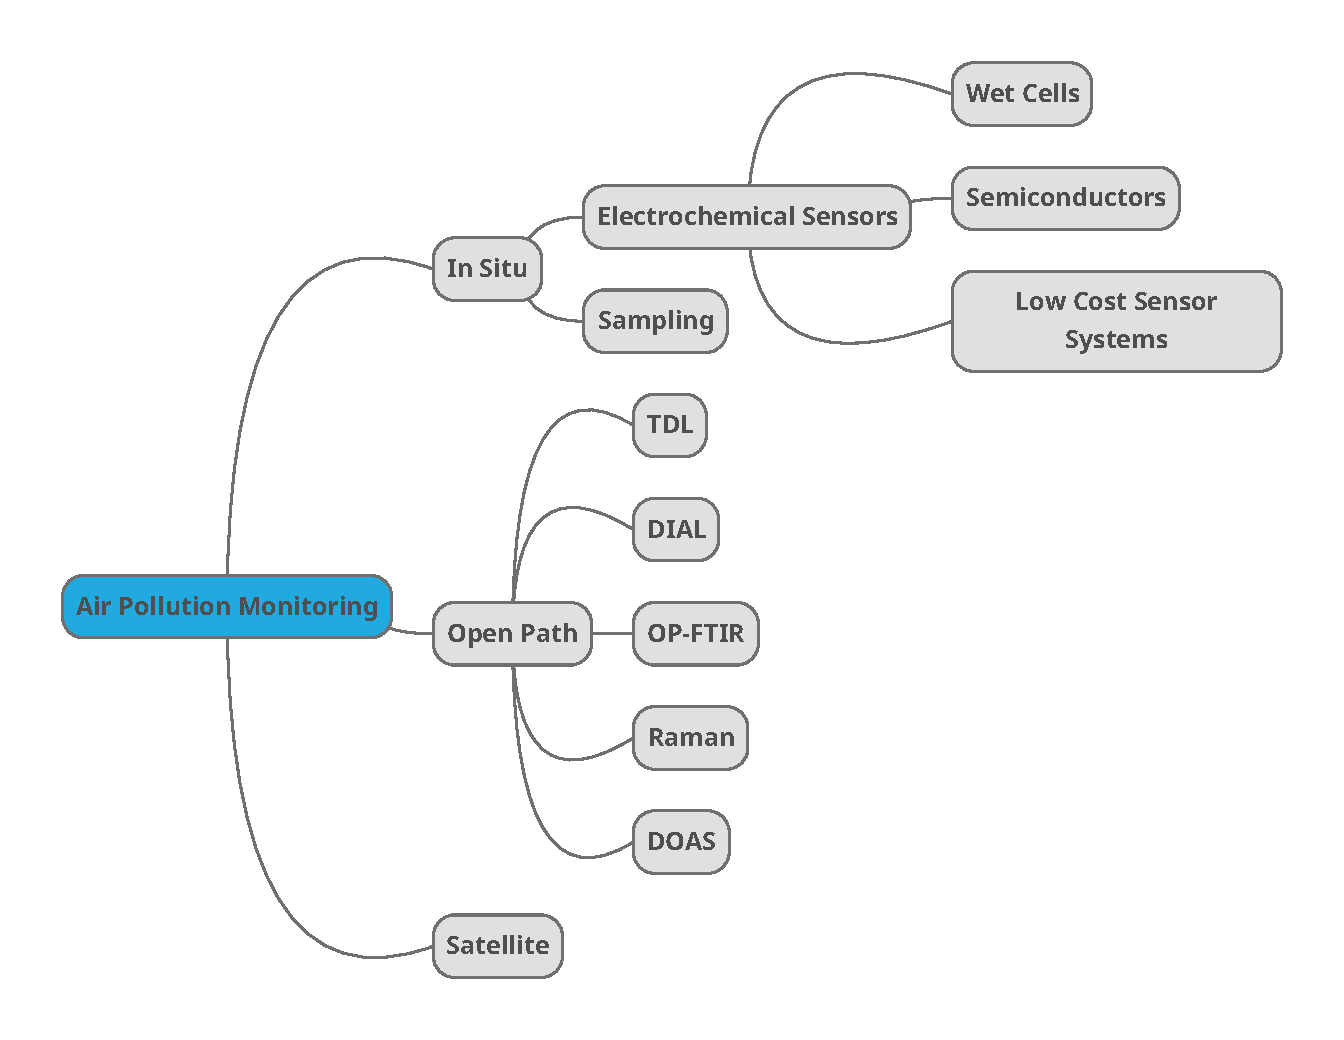
\includegraphics[width=.8\textwidth]{img/pdf/air_pollution_monitoring_tree.pdf}
%     \caption{A tree diagram providing a general overview of the various
%     types of atmospheric pollution monitoring systems. }%
%     \label{fig:pollution_monitoring_tree}
% \end{figure}

Sampling studies are still regarded as the gold standard for atmospheric
pollution monitoring. They are fundamentally different from the other
methods, because there is an important time gap between collection and
analysis. Sampling methods cannot provide real time information on
atmospheric composition. The gaseous analyte is moved into a collection
medium before being transported to the laboratory, where a very powerful
analytical method such as mass spectroscopy or chromatography is used to
retrieve the chemical composition of the sample. The use of this kind of
technique determines the importance of sampling methods in the study of
the atmosphere's composition, but they also make them quite inconvenient
for day to day use~\cite{Vallero2014}.

A much more convenient solution comes in the shape of electrochemical
sensors. They were highly popularised in recent decades through their
usage in the field of industrial hygiene~\cite{Clark1997}. The first
generation of these sensors were called wet cells. The basic design for
an \gls{o2} sensor of this type is presented in
Figure~\ref{fig:electrochemical_wet_cell}. When an electromagnetic force
is applied to the cell, hydrogen appears at the cathode, and oxygen at
the anode. Conversely, when the cathode is subject to an oxygen
concentration and an appropriate electrolyte is used (for instance,
KOH), an electronic charged develops through the oxidation of the anode
into a hydroxide. If a load is presented to the system, the current
flowing through it is proportional to the partial pressure of oxygen in
the mixture~\cite{Dhall2021, Clark1997}.

\begin{figure}[htpb]
    \centering
    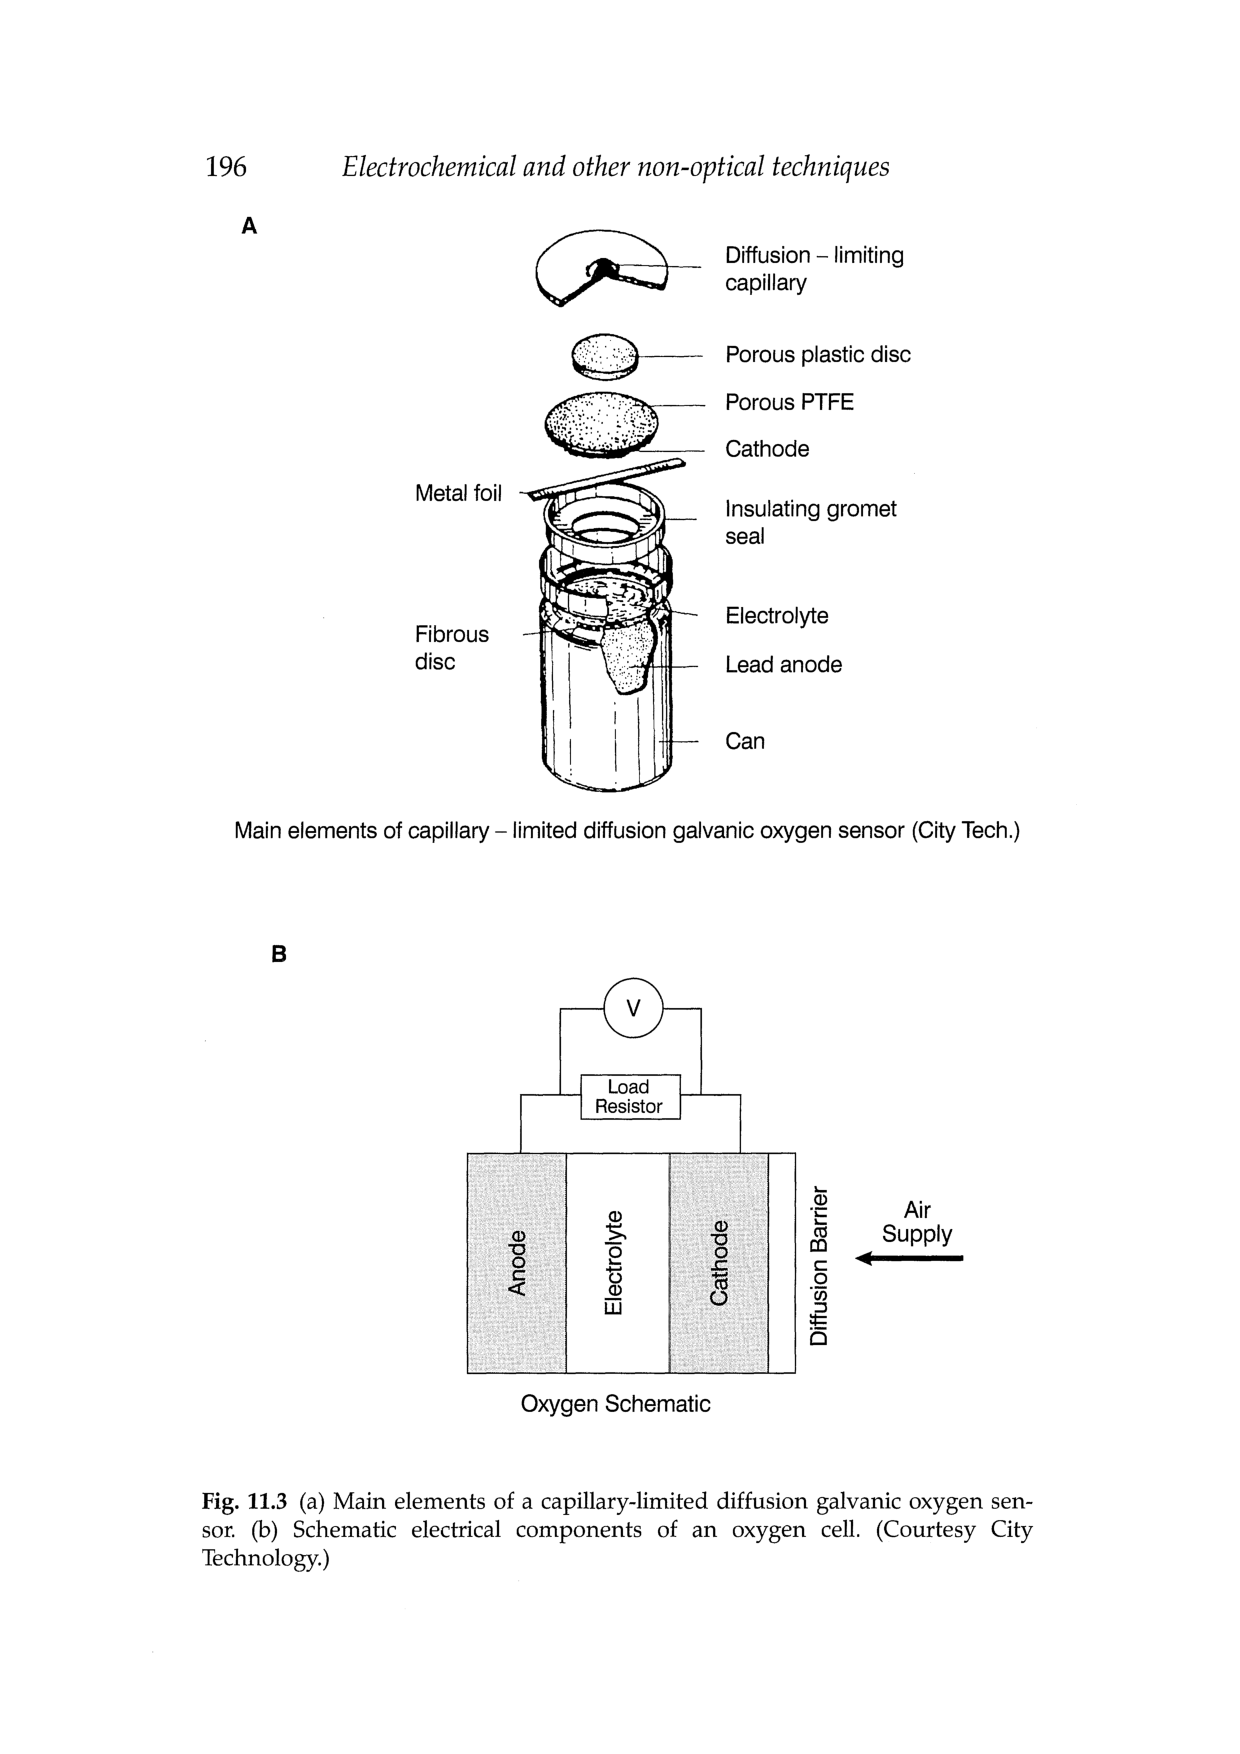
\includegraphics[trim=6cm 6.2cm 4cm 16cm, clip]{img/pdf/clark_193.pdf}
    \caption{General schematic for an electrochemical sensor cell by
    City Technology~\cite{Clark1997}.}%
    \label{fig:electrochemical_wet_cell}
\end{figure}

A similarly applicable technology is the use of semiconductor sensors.
These usually operate by the detection of a change in an electrical
characteristic of the sensor's material. These sensors usually display
sub-ppm detection limits, are easy to manufacture and to install and
have simple high-level operating principles (although some of them are
based on unknown phenomena~\cite{Dhall2021}). They are
also extremely cheap due to their needing minute quantities of sensing
materials. The most common approach to the semiconductor sensors is the
chemoresistive sensor. This sensor's resistance changes with the
presence of the target gas. They are based in the work of Brattain and
Bardeen~\cite{Dhall2021, Brattain1952}, in 1953. In spite of their many
advantages, semiconductor sensors also have their limitations. For
instance they are not as stable as most other measurement techniques.
They are also quite limited in terms of their selectivity, and therefore
should not be used in environments in which accuracy is a requirement.
Besides, they suffer from the fact that they are only meant to detect
what is directly in their vicinity, which means that they are easily
influenced by local sources (think of a car's exhaust near to the
sensor) which can mislead operators with regard to the atmosphere's
composition.

Open path atmospheric monitoring techniques are completely different.
Instead of relying in networks of small, local sensors, open-path
measurement methods apply optical principles to assess the atmosphere's
composition in a large area (up to a radius of a few km). \gls{tdl} is
one of such techniques, and one of the most popular. The measurement is
focused on a single line of the absorption spectrum of a particular
chemical species, to which \emph{the} laser is tuned. \gls{tdl} can be
used to retrieve data from several gaseous pollutants at the same time.
It is very user friendly, does not require any type of complex
maintenance and it is reasonably easy to implement. However, since the
laser is tuned to a particular wavelength, it has the important drawback
of needing one laser per target component. Moreover, only a relatively
limited set of components can be detected through this method, and
\gls{PM} and airborne objects are known to interfere with measurements
from this technique~\cite{Vallero2014, Kim2007}.

\gls{dial} is another important open-path technique. It uses \gls{lidar}
in two different wavelengths and measures the difference in absorption
between the two echos to determine the target gas concentration. By
measuring response times, \gls{dial} is also able to determine the
spatial distribution of the gas that is being measured. With regards to
drawbacks, there is a frequent problem with spectral artifacts that can
introduce some bias towards high densities (real concentrations are
smaller than they appear). Moreover, \gls{dial} depends on the lasers
that are used, so it can have a limited range of detected
components~\cite{Vallero2014}.

Infrared radiation can also be used to measure atmospheric gas
densities. The \gls{ftir} method (general schematic presented in
Figure~\ref{fig:ap_monitoring_ftir}) uses an interferometric measurement
of infrared light to determine how much of a particular gas was in the
analysed column. This is a very accurate method of obtaining average
concentrations along a path. However, it can be quite expensive and is
certainly the most complicated method described here. Moreover, strong
infrared absorption by water in the atmosphere can lead to it not being
useful in high-humidity environments. Raman spectroscopy can be used in
these situations, but this method has a much lower resolution, due to
the much lower intensity of the relevant signal~\cite{Vallero2014}.

\begin{figure}[htpb]
    \centering
    %{<left> <lower> <right> <upper>}
    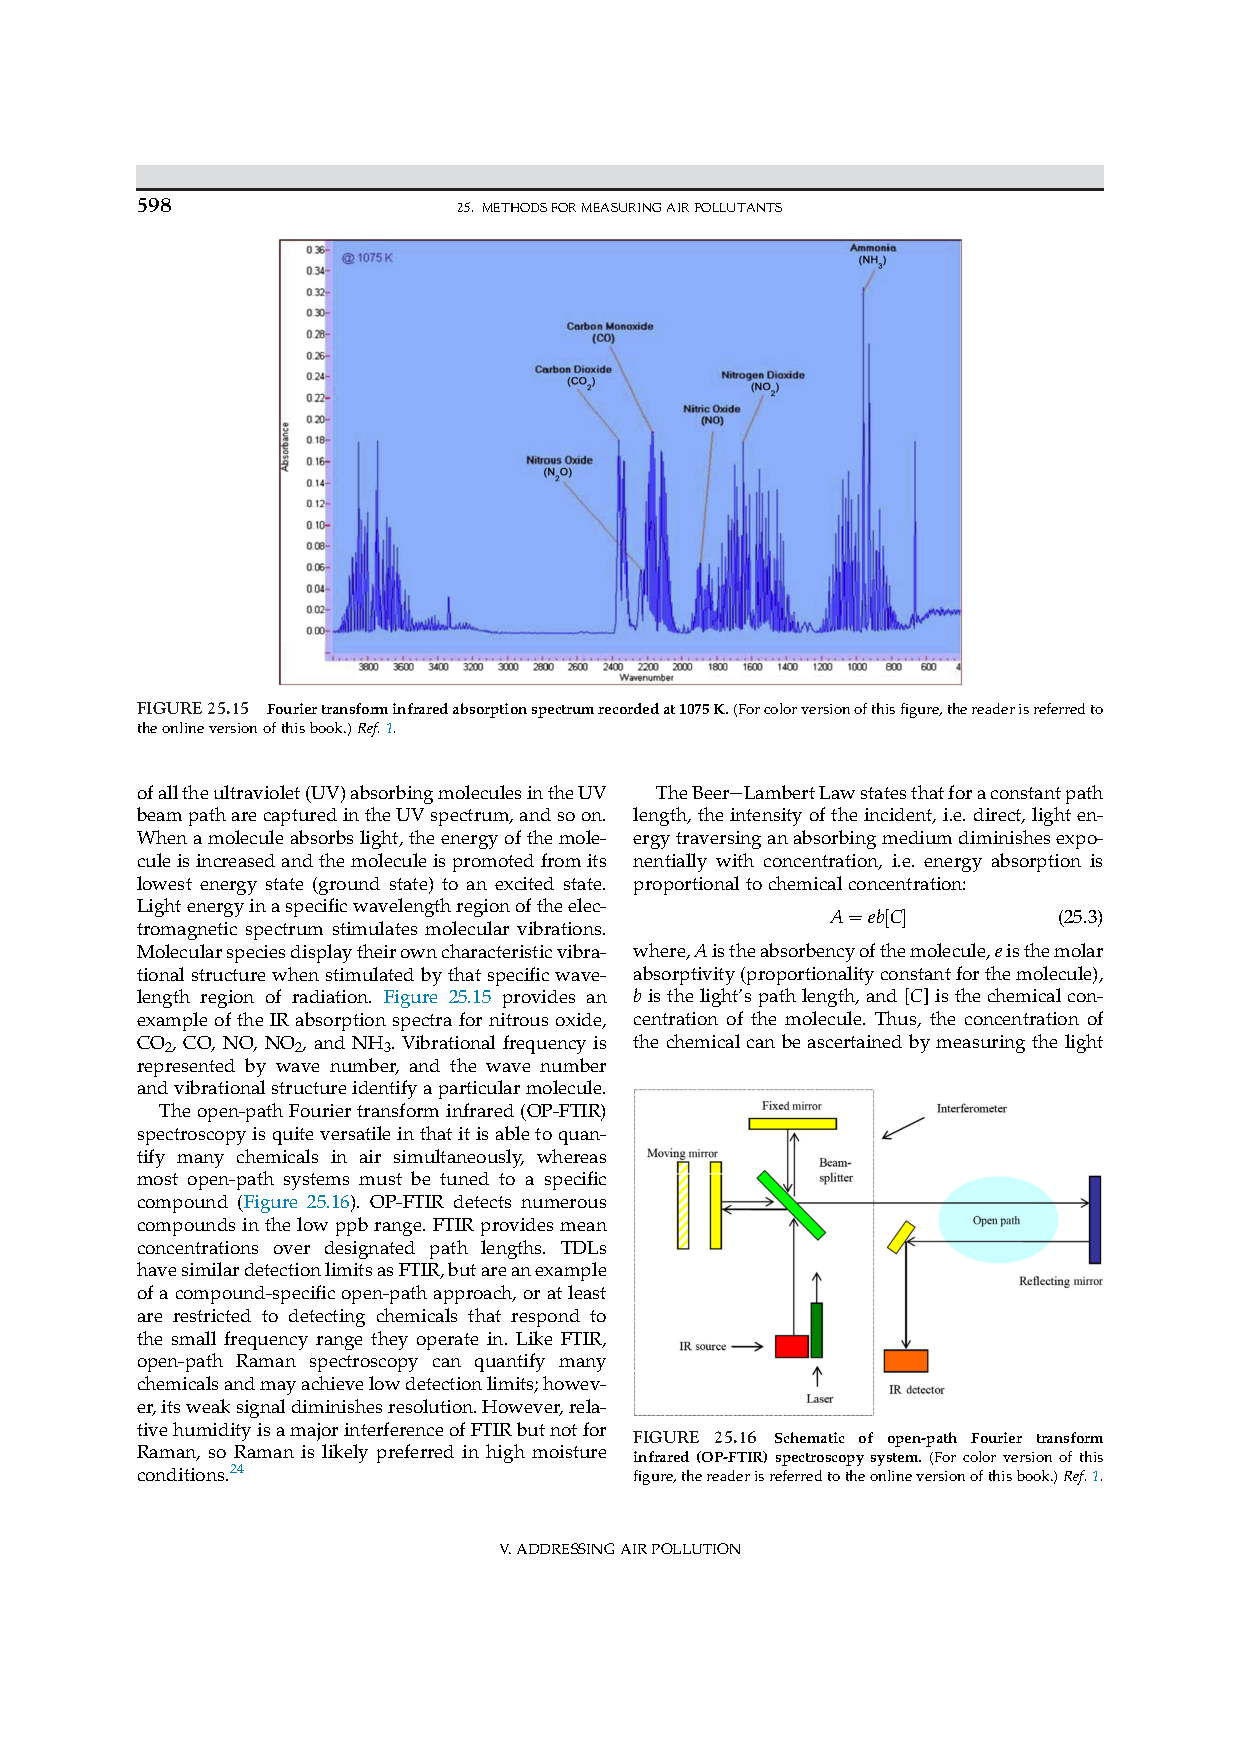
\includegraphics[trim=10.5cm 5.5cm 2cm 18cm,%...
        clip, frame, width=.8\textwidth]{img/pdf/vallero_ftir_588.pdf}
    \caption{General schematic of a \gls{ftir} instrument for
    atmospheric monitoring. Image adapted from~\cite{Vallero2014}.}%
    \label{fig:ap_monitoring_ftir}
\end{figure}

One of the most important atmospheric monitoring techniques available is
\gls{DOAS}. As \gls{ftir} and \gls{tdl}, \gls{DOAS} is based on
Lambert-Beer's law, so it determines the quantity of a given gas in the
atmosphere by how much light is absorbed on a certain light path and a
certain wavelength (which with \gls{DOAS}, can be a wavelength
interval). The method, which is explained in more detail in
Section~\ref{sec:doas} is able to simultaneously detect multiple trace
gases with ppm level accuracy (depending on the assembly). A \gls{DOAS}
system is a very easy to operate system, since once it is assembled it
requires no complicated maintenance.

The last atmospheric monitoring solution that I wish to delve on are
satellite-based techniques. In the last decade, we have seen a global
effort on behalf of governments (and transnational entities) to invest in
tools that can accurately monitor how atmospheric composition varies and
evolves through time. The EU developed the Copernicus network, with
several instruments already in orbit and Copernicus 5 scheduled for
launch in 2023; South Korea has deployed its Geostationary Environment
Monitoring Spectrometer in 2020, covering most of South-East Asia; and
the USA are preparing to launch their Tropospheric Emissions: Monitoring
of Pollution device in 2022. Together, this constellation of satellites
will provide hourly data from the most important pollution sources in
the world (example \gls{no2} map displayed in
Figure~\ref{fig:ap_monitoring_copernicus}). The amount and quality of
data that will come from these initiatives is something unheard of until
now, and has the potential to revolutionise how humans look at
tropospheric emissions. However, these applications lack spatial and
temporal resolution, as it is common for space-based terrestrial
monitoring instruments. Moreover, in spite of its total availability
(you can consult data on the internet), raw satellite data can be hard
to interpret and most of the times requires special knowledge and tools.

\begin{figure}[htpb]
    \centering
    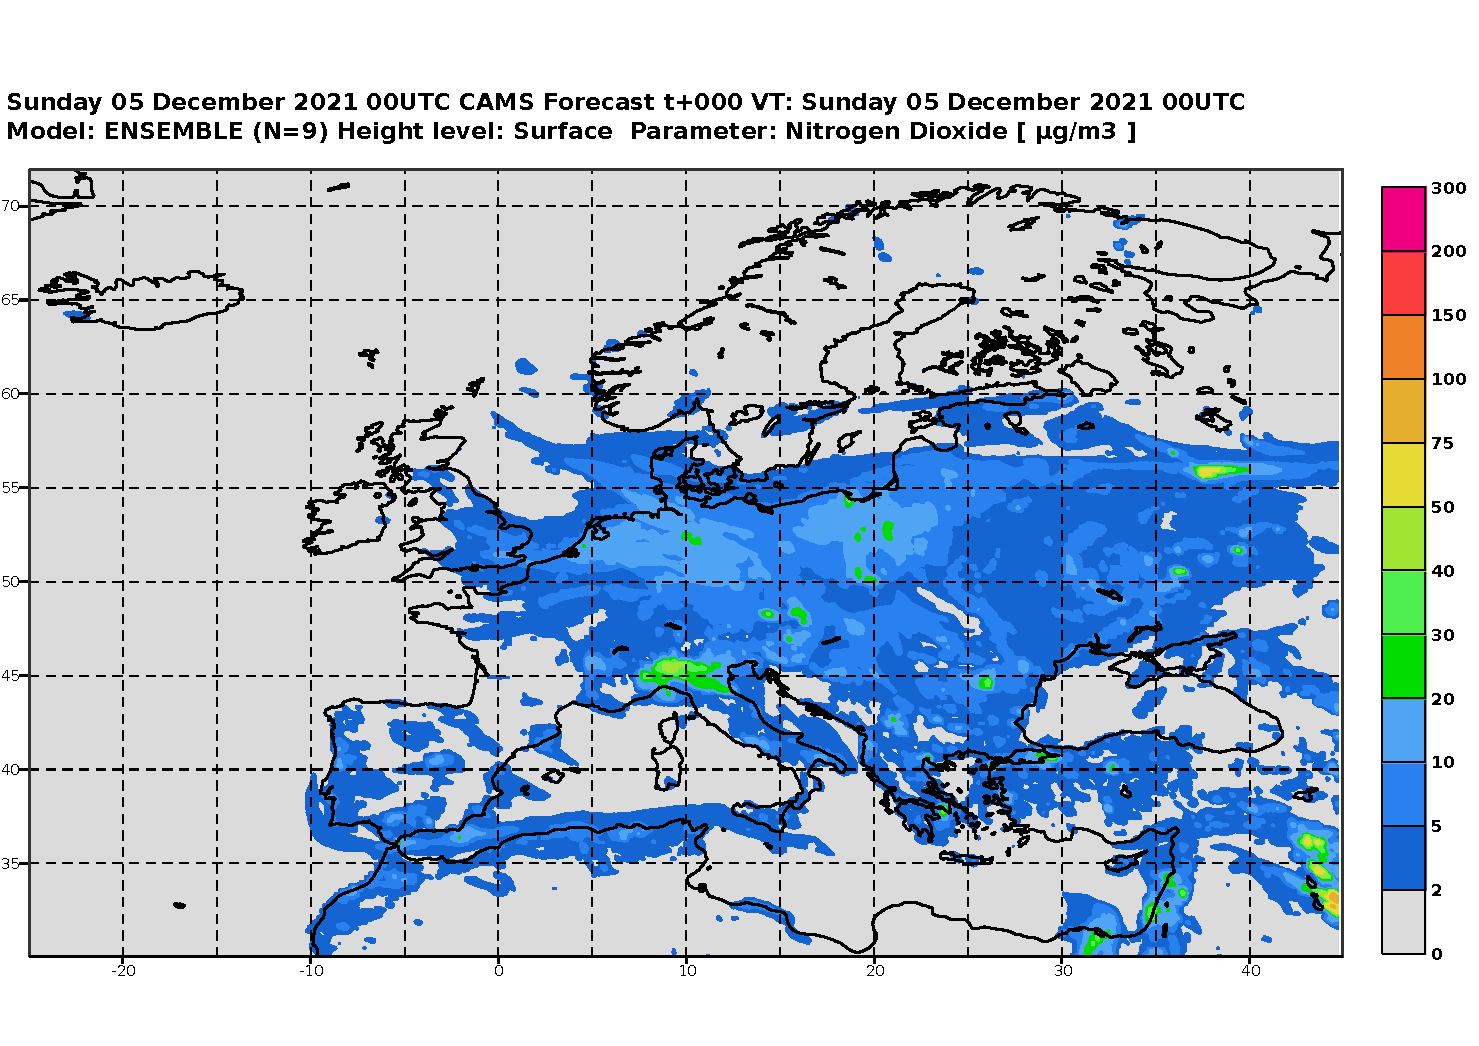
\includegraphics[width=.8\textwidth]{img/pdf/ENSEMBLE_no2_2021120500_SFC_000.pdf}
    \caption{Satellite \gls{no2} measurements over Europe. Figure taken
    from Copernicus's website~\cite{copernicusweb2021}.}%
    \label{fig:ap_monitoring_copernicus}
\end{figure}

Summarising, we have already several ways of monitoring, quantifying and
studying pollution. It is clear that one of the ways in which this field
of study will progress is through technology, namely through the
development of new intelligent instruments that \emph{fill the blanks}
that are currently left by what we can use today~\cite{EEA2019,
Kim2007}. At this point I would point out to the reader the summary
table that is presented in Table~\ref{tab:ap_monitoring_summary_table}.
The amount of green in it should be an inspiring sight. Most methods are
generally very useful. However, \gls{DOAS} has a single red cell,
corresponding to spatial resolution. While this is a limitation of the
\emph{vanilla} \gls{DOAS} method, it does not hold for some of this
technique's more recent ramifications. In fact, \gls{DOAS} tomography
can very well solve this problem. This was the rationale behind the path
that was chosen in this thesis' work, and the motto for the rest of this
document.

\begin{table}[htb]
\centering
\caption{Summary table for \gls{AP} monitoring methods. Highlighted are
perceived strengths and weaknesses: \textcolor{red}{red} for bad,
\textcolor{green}{green} for good. In this table, electrochemical
sensors are abbreviated to EC and semiconductor sensors to SC.}
\label{tab:ap_monitoring_summary_table}
\small
\begin{tabularx}{\textwidth}{XXXXcXXX}
    \toprule
\textbf{Method}          & \textbf{Acc.}
                         & \textbf{Temp. Res.}
                         & \textbf{Spt. Res.}
                         & \textbf{Robustness}                                & \textbf{Ease of Use}                                  & \textbf{Cost over time}                               \\ \midrule
\textbf{Sampling}        & \cellcolor[HTML]{C6EFCD}{\color[HTML]{367E33} High}   & \cellcolor[HTML]{FFC7CE}{\color[HTML]{9C006E} Low}  & \cellcolor[HTML]{C6EFCD}{\color[HTML]{367E33} High} & \cellcolor[HTML]{FFEB9C}{\color[HTML]{AA6A17} Medium} & \cellcolor[HTML]{FFC7CE}{\color[HTML]{9C006E} Low}    & \cellcolor[HTML]{C6EFCD}{\color[HTML]{367E33} Low}    \\
\textbf{EC} & \cellcolor[HTML]{FFC7CE}{\color[HTML]{9C006E} Low}    & \cellcolor[HTML]{C6EFCD}{\color[HTML]{367E33} High} & \cellcolor[HTML]{C6EFCD}{\color[HTML]{367E33} High} & \cellcolor[HTML]{FFC7CE}{\color[HTML]{9C006E} Low}    & \cellcolor[HTML]{C6EFCD}{\color[HTML]{367E33} High}   & \cellcolor[HTML]{FFC7CE}{\color[HTML]{9C006E} High}   \\
\textbf{SC}  & \cellcolor[HTML]{FFC7CE}{\color[HTML]{9C006E} Low}    & \cellcolor[HTML]{C6EFCD}{\color[HTML]{367E33} High} & \cellcolor[HTML]{C6EFCD}{\color[HTML]{367E33} High} & \cellcolor[HTML]{FFC7CE}{\color[HTML]{9C006E} Low}    & \cellcolor[HTML]{C6EFCD}{\color[HTML]{367E33} High}   & \cellcolor[HTML]{FFEB9C}{\color[HTML]{AA6A17} Medium} \\
\textbf{\gls{tdl}}       & \cellcolor[HTML]{C6EFCD}{\color[HTML]{367E33} High}   & \cellcolor[HTML]{C6EFCD}{\color[HTML]{367E33} High} & \cellcolor[HTML]{FFC7CE}{\color[HTML]{9C006E} Low}  & \cellcolor[HTML]{C6EFCD}{\color[HTML]{367E33} High}   & \cellcolor[HTML]{FFEB9C}{\color[HTML]{AA6A17} Medium} & \cellcolor[HTML]{C6EFCD}{\color[HTML]{367E33} Low}    \\
\textbf{\gls{dial}}      & \cellcolor[HTML]{FFEB9C}{\color[HTML]{AA6A17} Medium} & \cellcolor[HTML]{C6EFCD}{\color[HTML]{367E33} High} & \cellcolor[HTML]{FFC7CE}{\color[HTML]{9C006E} Low}  & \cellcolor[HTML]{C6EFCD}{\color[HTML]{367E33} High}   & \cellcolor[HTML]{FFC7CE}{\color[HTML]{9C006E} Low}    & \cellcolor[HTML]{C6EFCD}{\color[HTML]{367E33} Low}    \\
\textbf{\gls{ftir}}      & \cellcolor[HTML]{C6EFCD}{\color[HTML]{367E33} High}   & \cellcolor[HTML]{C6EFCD}{\color[HTML]{367E33} High} & \cellcolor[HTML]{FFC7CE}{\color[HTML]{9C006E} Low}  & \cellcolor[HTML]{C6EFCD}{\color[HTML]{367E33} High}   & \cellcolor[HTML]{FFC7CE}{\color[HTML]{9C006E} Low}    & \cellcolor[HTML]{FFC7CE}{\color[HTML]{9C006E} High}   \\
\textbf{\gls{DOAS}}      & \cellcolor[HTML]{C6EFCD}{\color[HTML]{367E33} High}   & \cellcolor[HTML]{C6EFCD}{\color[HTML]{367E33} High} & \cellcolor[HTML]{FFC7CE}{\color[HTML]{9C006E} Low}  & \cellcolor[HTML]{C6EFCD}{\color[HTML]{367E33} High}   & \cellcolor[HTML]{C6EFCD}{\color[HTML]{367E33} High}   & \cellcolor[HTML]{C6EFCD}{\color[HTML]{367E33} Low}    \\
\textbf{Satellite}       & \cellcolor[HTML]{C6EFCD}{\color[HTML]{367E33} High}   & \cellcolor[HTML]{FFC7CE}{\color[HTML]{9C006E} Low}  & \cellcolor[HTML]{FFC7CE}{\color[HTML]{9C006E} Low}  & \cellcolor[HTML]{C6EFCD}{\color[HTML]{367E33} High}   & \cellcolor[HTML]{FFEB9C}{\color[HTML]{AA6A17} Medium} & \cellcolor[HTML]{C6EFCD}{\color[HTML]{367E33} Low}    \\ \bottomrule
\end{tabularx}
\end{table}

